% $Header: /home/vedranm/bitbucket/beamer/solutions/conference-talks/conference-ornate-20min.en.tex,v 90e850259b8b 2007/01/28 20:48:30 tantau $

\documentclass{beamer}

% This file is a solution template for:

% - Talk at a conference/colloquium.
% - Talk length is about 20min.
% - Style is ornate.



% Copyright 2004 by Till Tantau <tantau@users.sourceforge.net>.
%
% In principle, this file can be redistributed and/or modified under
% the terms of the GNU Public License, version 2.
%
% However, this file is supposed to be a template to be modified
% for your own needs. For this reason, if you use this file as a
% template and not specifically distribute it as part of a another
% package/program, I grant the extra permission to freely copy and
% modify this file as you see fit and even to delete this copyright
% notice. 


\mode<presentation>
{
  \usetheme{BACL}
  % or ...

  \setbeamercovered{transparent}
  % or whatever (possibly just delete it)
}


\usepackage[english]{babel}
% or whatever

\usepackage[latin1]{inputenc}
% or whatever

\usepackage{times}
\usepackage[T1]{fontenc}
\usepackage{subfigure}
\usepackage{subfigmat}
\usepackage{hyperref}

% Or whatever. Note that the encoding and the font should match. If T1
% does not look nice, try deleting the line with the fontenc.


\title[] % (optional, use only with long paper titles)
{Comprehensive Exam Proposal}

\subtitle
{Moving Grids for Design CFD}

\author[C. Nathan Woods, R. Starkey] % (optional, use only with lots of authors)
{Nathan Woods \and Ryan Starkey}
% - Give the names in the same order as the appear in the paper.
% - Use the \inst{?} command only if the authors have different
%   affiliation.

\institute[CU-Boulder] % (optional, but mostly needed)
{
%  \inst{1}%
  Busemann Advanced Concepts Laboratory\\
  Department of Aerospace Engineering Sciences\\
  University of Colorado at Boulder}
%  \and
%  \inst{2}%
%  Department of Theoretical Philosophy\\
%  University of Elsewhere}
%% - Use the \inst command only if there are several affiliations.
%% - Keep it simple, no one is interested in your street address.

\date[] % (optional, should be abbreviation of conference name)
{1 December 2011}
% - Either use conference name or its abbreviation.
% - Not really informative to the audience, more for people (including
%   yourself) who are reading the slides online

%\subject{Theoretical Computer Science}
%% This is only inserted into the PDF information catalog. Can be left
%% out. 



% If you have a file called "university-logo-filename.xxx", where xxx
% is a graphic format that can be processed by latex or pdflatex,
% resp., then you can add a logo as follows:

% \pgfdeclareimage[height=0.5cm]{university-logo}{university-logo-filename}
% \logo{\pgfuseimage{university-logo}}

\pgfdeclareimage[height=1.25cm]{CUlogo}{CUlogo.pdf}
\logo{\pgfuseimage{CUlogo}}

% Delete this, if you do not want the table of contents to pop up at
% the beginning of each subsection:
\AtBeginSection[]
{
  \begin{frame}<beamer>{Outline}
    \tableofcontents[currentsection]%,currentsubsection]
  \end{frame}
}


% If you wish to uncover everything in a step-wise fashion, uncomment
% the following command: 

%\beamerdefaultoverlayspecification{<+->}


\begin{document}
\begin{frame}
  \titlepage
\end{frame}

%\begin{frame}{Outline}
%  \tableofcontents
%  % You might wish to add the option [pausesections]
%\end{frame}


% Structuring a talk is a difficult task and the following structure
% may not be suitable. Here are some rules that apply for this
% solution: 

% - Exactly two or three sections (other than the summary).
% - At *most* three subsections per section.
% - Talk about 30s to 2min per frame. So there should be between about
%   15 and 30 frames, all told.

% - A conference audience is likely to know very little of what you
%   are going to talk about. So *simplify*!
% - In a 20min talk, getting the main ideas across is hard
%   enough. Leave out details, even if it means being less precise than
%   you think necessary.
% - If you omit details that are vital to the proof/implementation,
%   just say so once. Everybody will be happy with that.

\section{Introduction}

\begin{frame}{About Me}
  Married Kristin Woods, 2010
  Places I've lived - Georgia, Texas, Utah, Iowa, Idaho, Colorado
  Schools I've attended:
  \begin{itemize}
  \item Richfield High School, Richfield, Utah - 2002
  \item Brigham Young University, Provo, Utah -  2008, B.S. Physics
  \item University of Colorado, Boulder, Colorado -  2013, Ph.D. Aerospace Engineering
  \end{itemize}
  Research I've been involved in:
    \begin{itemize}
    \item Direct Simulation Monte Carlo (DSMC) for high-temperature
      gas mixtures
    \item Fabrication of nano-sensors for Mars missions
    \item Design of a miniature turbojet engine
    \item Development and design of far-infrared optical sensors
    \end{itemize}
\end{frame}

\begin{frame}{About Me, con't}
My Interests (Technical \& Otherwise):
\begin{itemize}
  \item Theoretical \& computational physics
  \item Complex systems \& emergent behavior
  \item Application of advanced mathematics
  \item Performance home computing
  \item Home networking
  \item Running \& rock climbing
\end{itemize}
\end{frame}

\subsection{An Example Problem - Joint Strike Fighter ASTOVL Analysis}

\begin{frame}{Joint Strike Fighter ASTOVL Analysis}
  \begin{figure}
    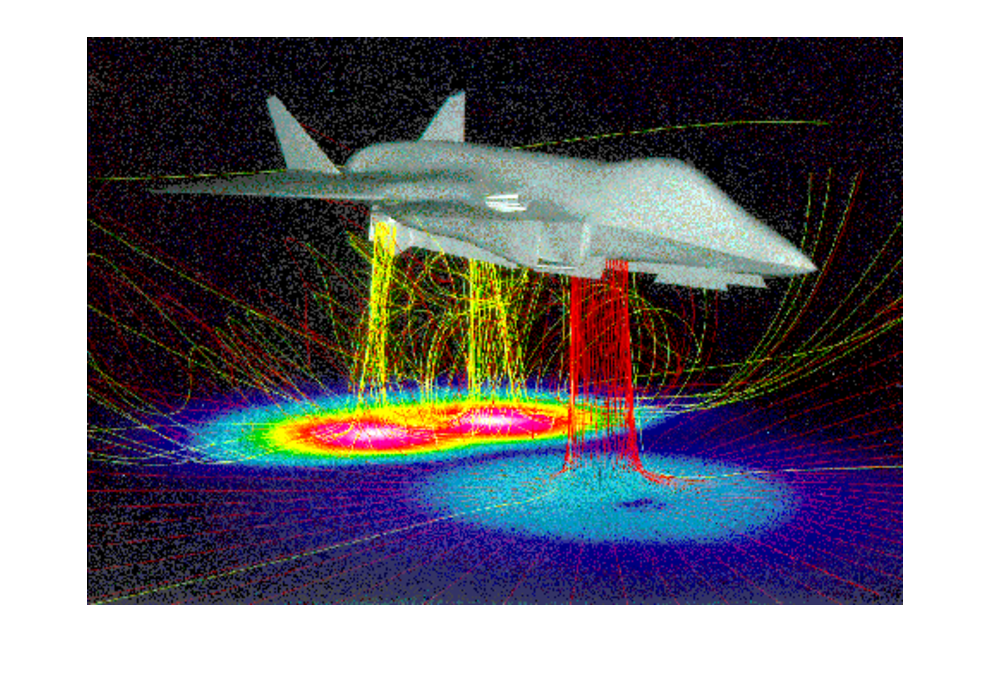
\includegraphics[width=.7\textwidth]{JSFStreams.pdf}
    \caption{Computed streamlines of the Joint Strike Fighter B variant during vertical landing. Ground plane colored by temperature. Courtesy of Pointwise, makers of Gridgen software - http://www.pointwise.com/apps/b2jsf.shtml}
%    \notes{There are three major problems with an ASTOVL design such as the JSF. Close ground effects can lead to negative lift, hot gas ingestion can dramatically reduce engine performance, and the hot, recirculating ``fountain'' generated can damage the skin of the aircraft. While a prototype had been tested in a wind tunnel, engineers felt that a computer simulation would streamline the design process.}
  \end{figure}
\end{frame}

\begin{frame}{Joint Strike Fighter ASTOVL Analysis}
  \begin{figure}
    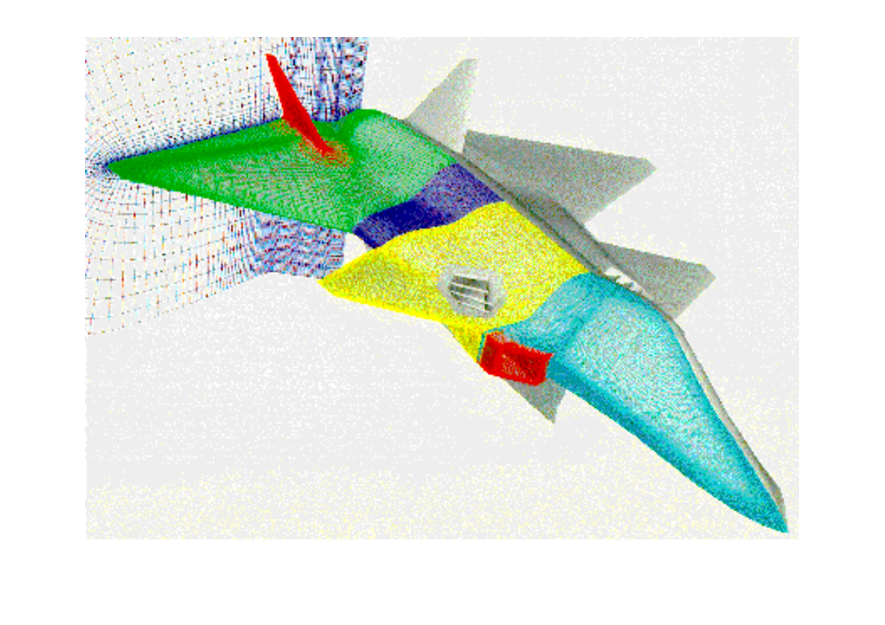
\includegraphics[width = .7\textwidth]{JSFGrid.pdf}
    \caption{Top view of grid used in above JSF analysis, showing various structured grid blocks.}
%    \notes{Northrup Grumman engineers used Gridgen, an advanced preprocessor designed in cooporation with NASA, to generate a block-structured computational mesh from  a NASA IGES file. The process, as described by Pointwise, the makers of Gridgen, is as follows: Manually define block boundaries: connectors, surfaces, and blocks. Generate grid points along connectors using a user specified distribution. Iteratively smooth the grid to ensure positive cell volume and other desireable features. This process took several hours for trained Northrup Grumman engineers, using top-of-the-line commercial software, with which they were presumably familiar. The CFD analysis took about 60 hours on a NASA Ames supercomputer and returned well-correlated results. Now, imagine trying to scale this problem to the level of preliminary design.}
  \end{figure}
\end{frame}

\subsection{CFD for Design}

\begin{frame}{The Project Cycle}
  \begin{figure}
    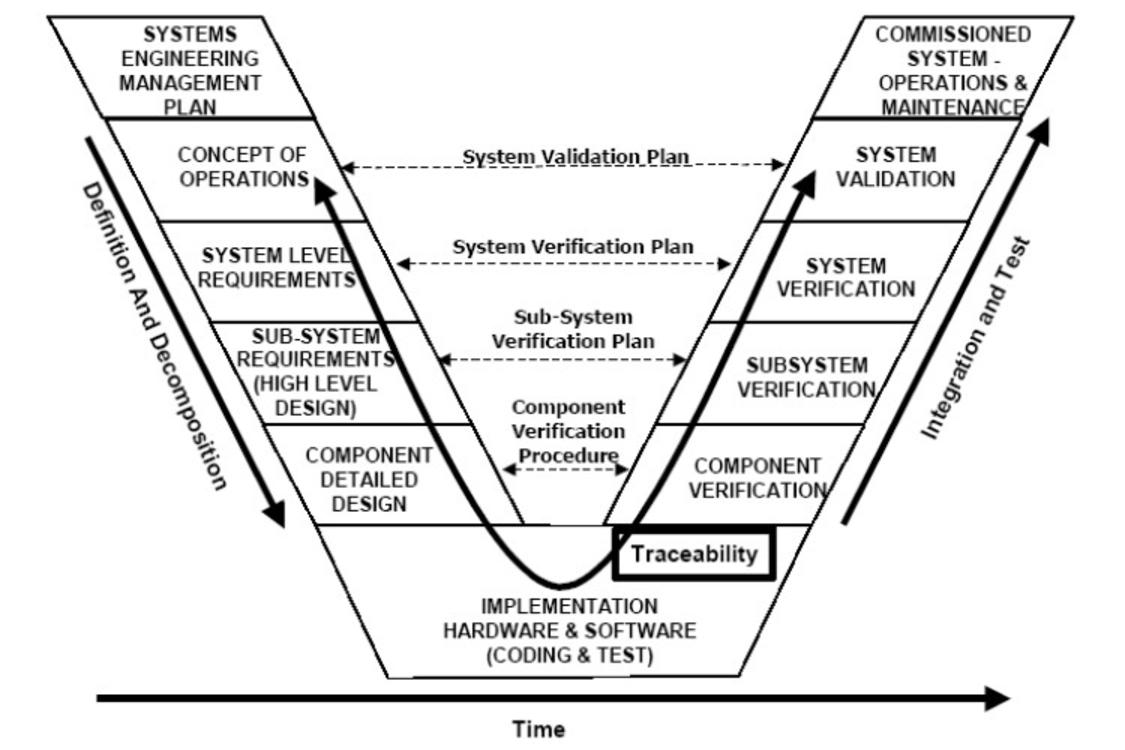
\includegraphics[height=2in]{Systems_Engineering_V_diagram.pdf}
    \caption{The life cycle of a project.
    (Wikimedia Commons)
%, taken from {\em Systems Engineering for Intelligent Transportation Systems}, Washington State Department of Transportation
}
%    \notes{To quote Dr. Jameson of Stanford, ``CFD is still not being exploited as effectively as one would like in the design process. This is partially because of the long set-up times and high costs, both human and computational, of complex flow simulations.''}
  \end{figure}
\end{frame}

\begin{frame}{The Project Cycle}
  \emph{``CFD is still not being exploited as effectively as one would like
    in the design process. This is partially because of the long set-up
    times and high costs, both human and computational, of complex flow
  simulations.''}  -- Antony Jameson, Stanford, 1999 \vspace{.25in}

\emph{``The conceptual design stage is the point where the most 
freedom is available to change the design...
%, thereby allowing CFD to make the largest impact. However, 
normally, 
advanced CFD tools aren't used until the start of preliminary 
design at the earliest.''} -- William Mason, Virginia Tech, 1998
\end{frame}

\begin{frame}{Requirements for Design CFD}
  Essential characteristics of a CFD design tool are:
  \begin{itemize}
  \item Short set-up times
  \item Low computational costs
  \end{itemize}
  \vspace{.25in}
  We believe the unified coordinate system 
  \href{http://www.youtube.com/watch?v=g-a9oGpKiEw}{[link]}
  will help with both of these requirements.
\end{frame}

% \begin{frame}{Reducing Costs - The Unified Coordinates}
% \begin{itemize}
% \item Quick tests for new designs
% \item No grid generation
% \item Automatic refinement
% \end{itemize}
% \end{frame}

%\begin{frame}{Lagrangian CFD \& Unified Coordinates}
%  The Unified Coordinates
%\end{frame}

\begin{frame}{The Unified Coordinate System}
  \begin{itemize}
    \item Lagrangian Fluid dynamics
      \vspace{.025in}
      \begin{itemize}
        \item Automatic grid generation
        \item Can fail due to severe grid distortion
      \end{itemize}
      \vspace{.025in}
    \item Unified Coordinates
      \vspace{.025in}
      \begin{itemize}
        \item Largely preserves benefits of Lagrangian systems
        \item Distortion can be controlled
      \end{itemize}
  \end{itemize}
  \begin{figure}
    \vspace{.125in}
    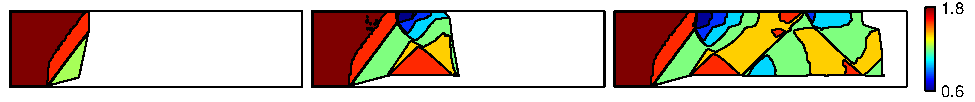
\includegraphics[width=\textwidth]{Channel_flow_filmstrip_image_mach.pdf}
    \caption{Mach contours for a transonic duct flow}
  \end{figure}
\end{frame}

\subsection{Previous Work}
% Talk about when and by whom this work was done. Include images for
% recirculation 
% Talk a little about Hui's background as APPM
\begin{frame}{Original Development of UCS}
  Developed by W. H. Hui\cite{hui07} from from Lagrangian coordinates
  \vspace{.025in}
    ``I wish I had developed this at the beginning of my career,
    rather than at the end'' - W. H. Hui, 2000, personal communication
  \begin{itemize}
   \vspace{.025in}
    \item The time-dependent Euler equations\cite{hui99}\cite{hui01}
    \item Extension to viscous flows\cite{huiviscous07}
    \item External flows and oscillating airfoils\cite{hui04}$^,$\cite{huigridless}
  \end{itemize}
\end{frame}

\begin{frame}{Original Development of UCS}
  \begin{figure}
    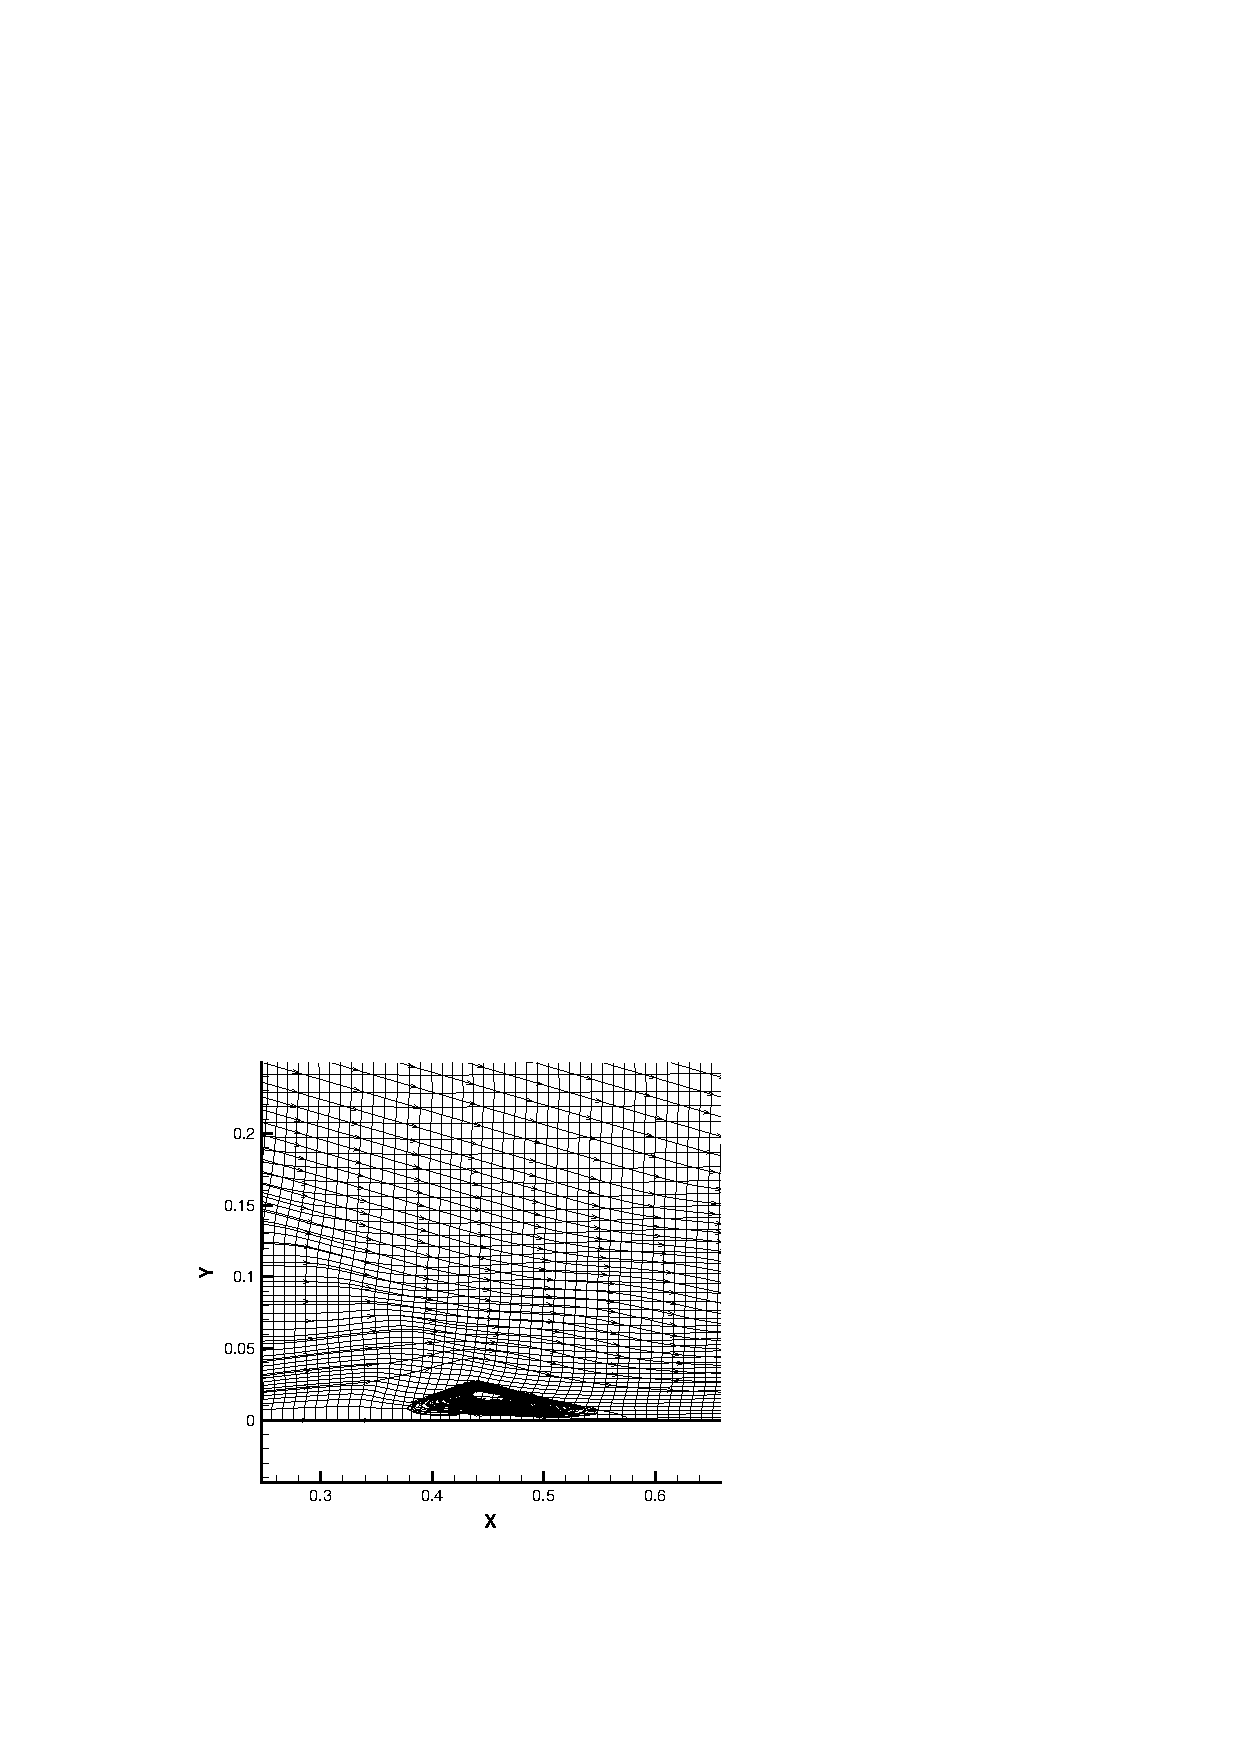
\includegraphics[height=.7\textheight]{ViscousRecirculationStreamsHui.pdf}
    \caption{Boundary-layer separation \& recirculation in
      Navier-Stokes equations captured by UCS\cite{huiviscous07}}
  \end{figure}
\end{frame}

\begin{frame}{Original Development of UCS}
  \begin{figure}
    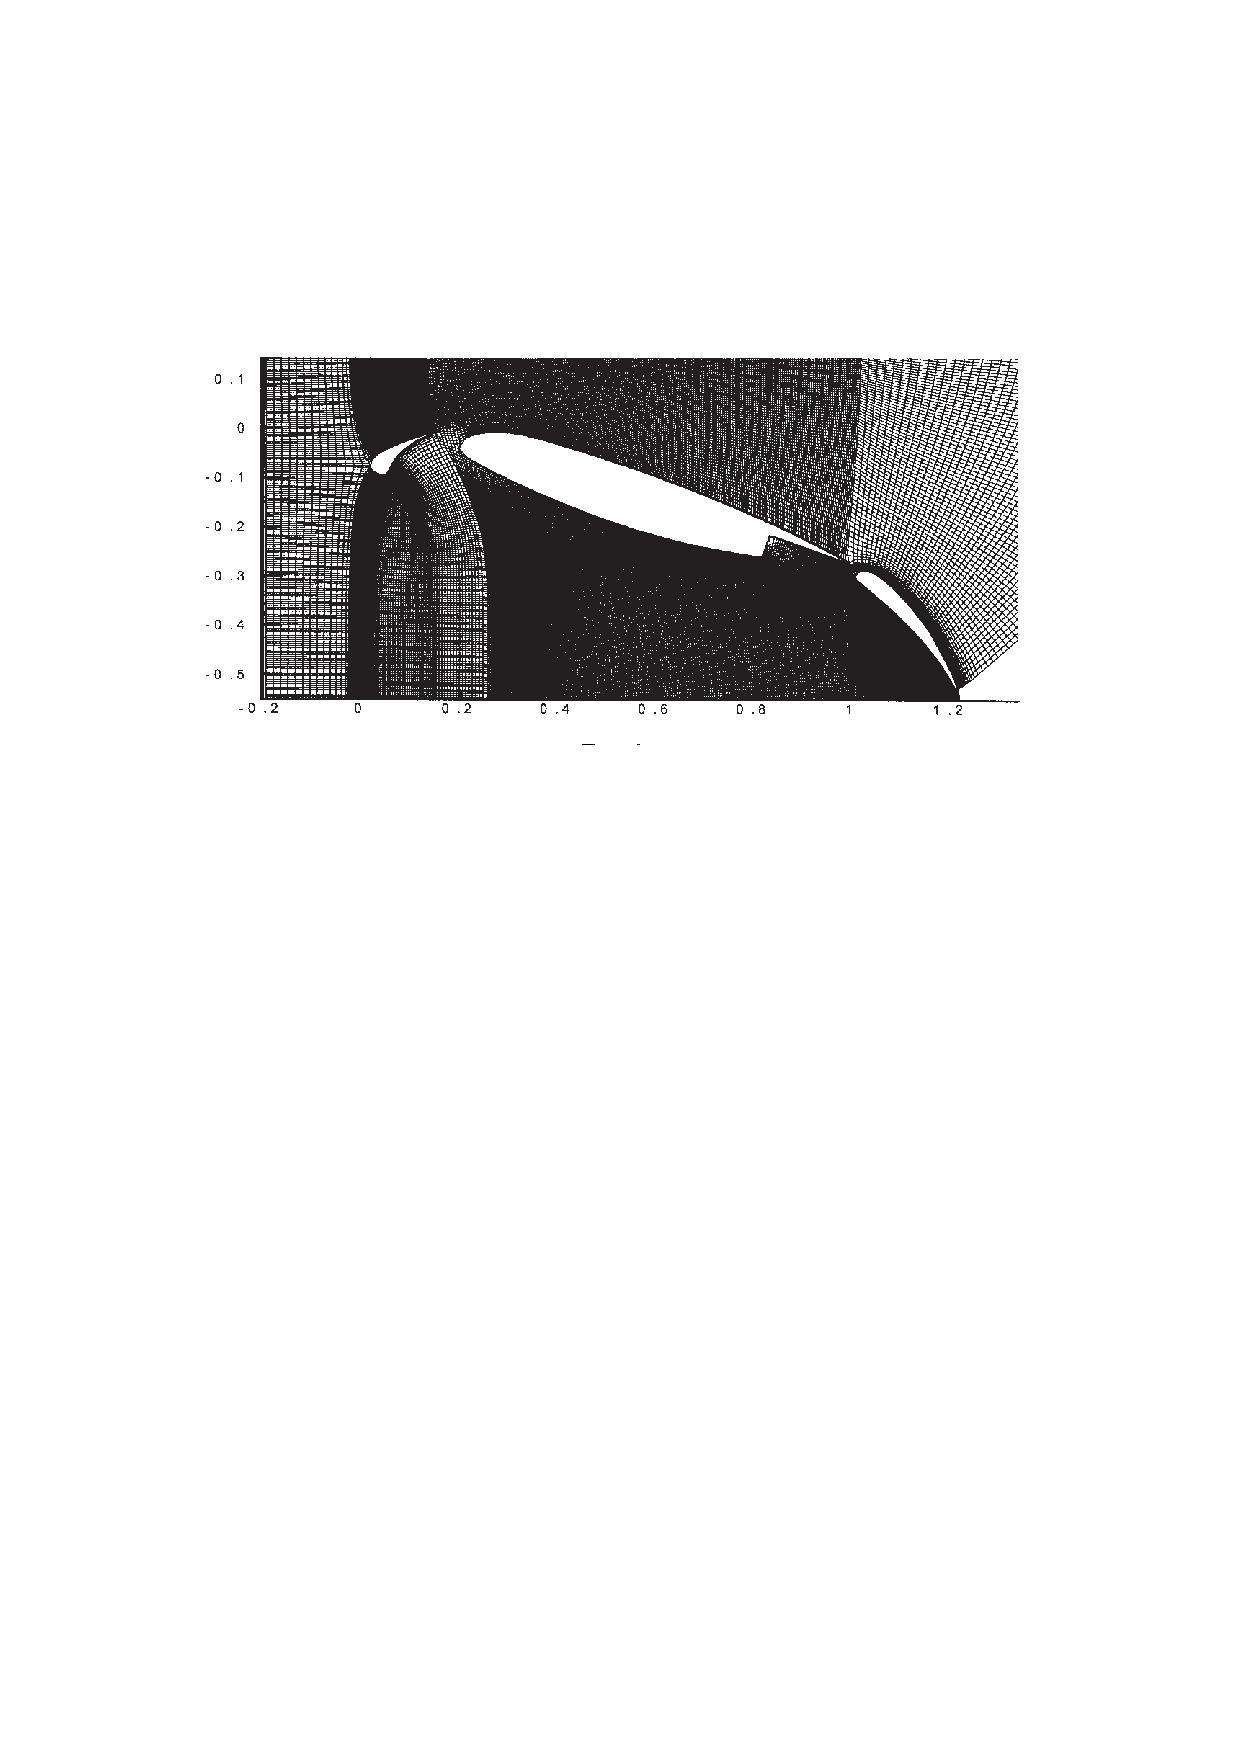
\includegraphics[width=\textwidth]{MultiElementAirfoilGrid.pdf}
    \caption{A complex unified grid generated by Hui\cite{huimulti}}
  \end{figure}
\end{frame}

\begin{frame}{Extensions of UCS}
  Applications of UCS to other systems
  \vspace{.025in}
  \begin{itemize}
    \item Multimaterial flows\cite{jia06}
    \item Plasma dynamics\cite{zhilkin07}
    \item Gas-kinetic (BGK) aerodynamics\cite{jin07}
  \end{itemize}
\end{frame}

\begin{frame}
  \begin{figure}
    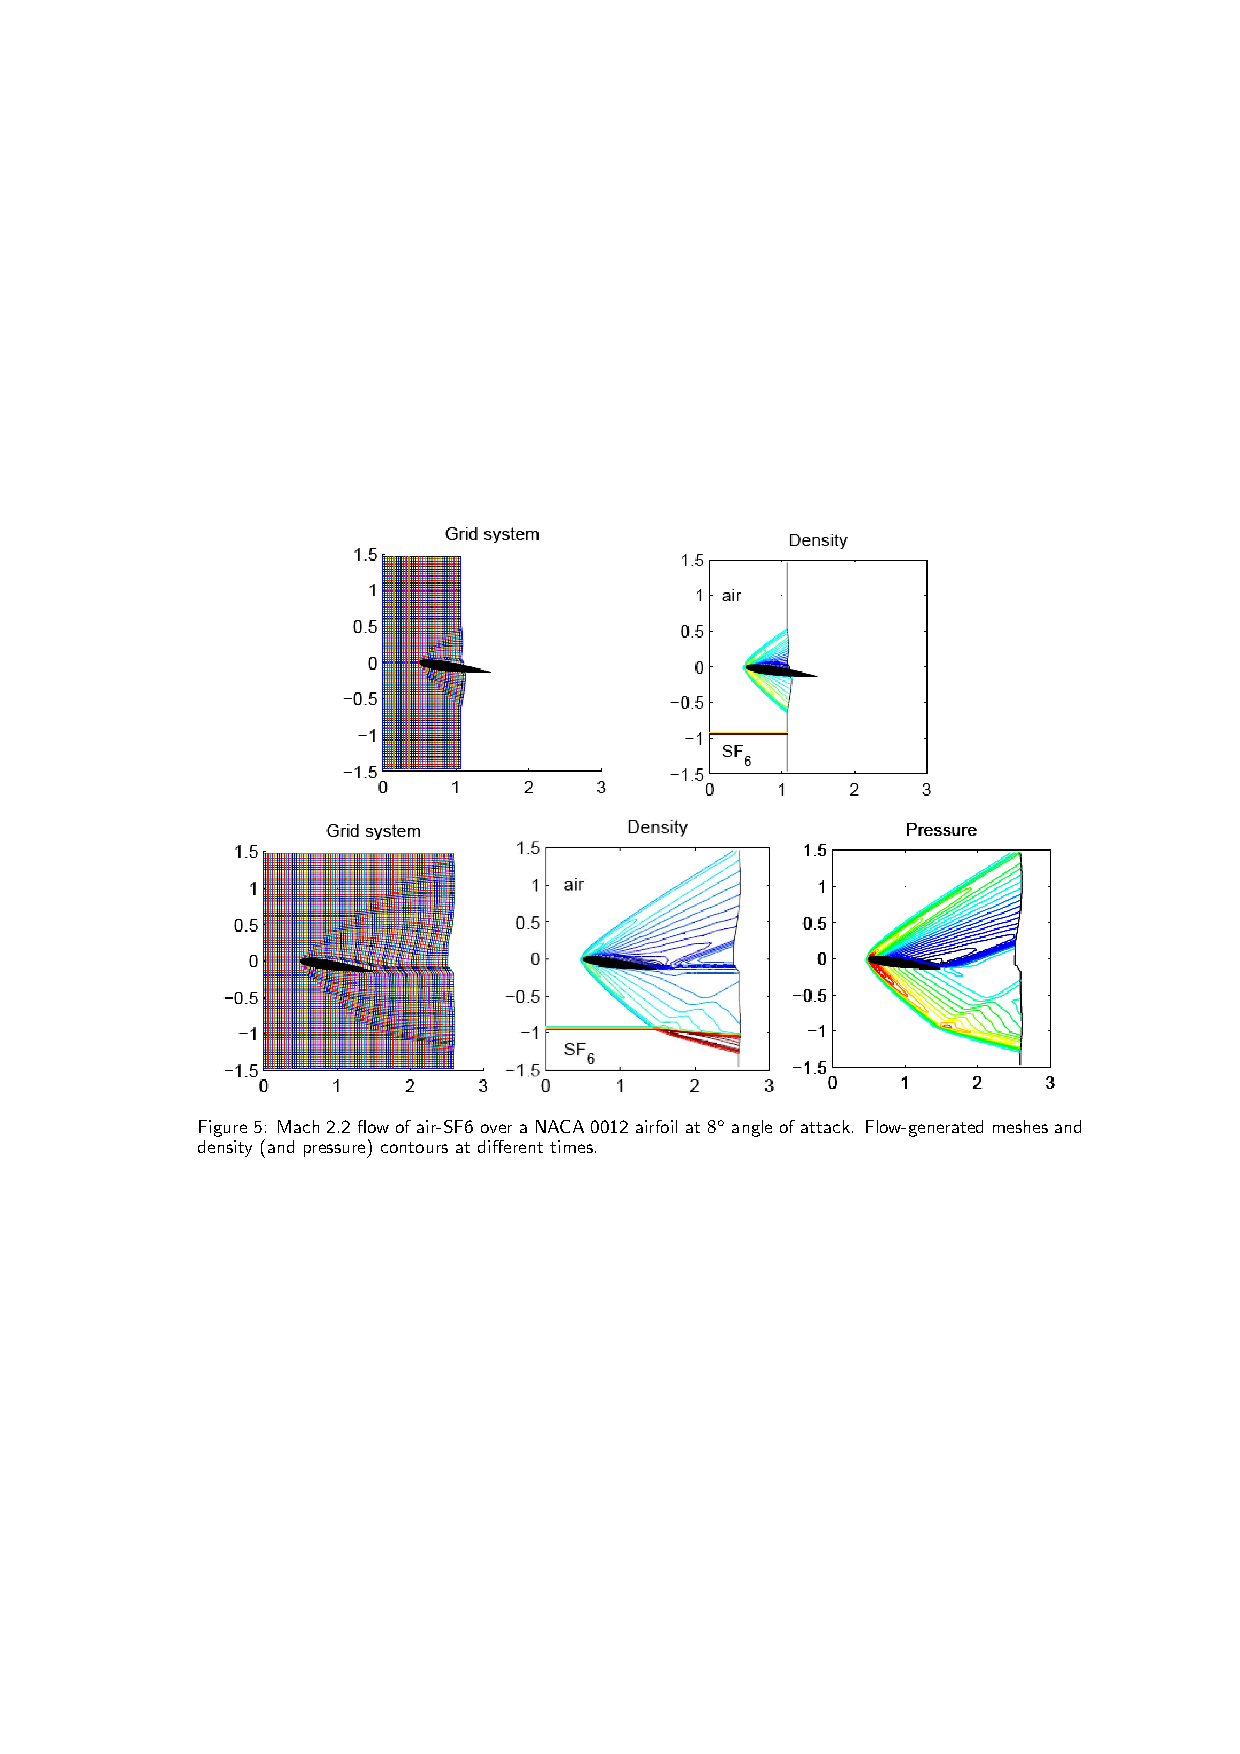
\includegraphics[width=\textwidth]{MultiMaterialAirfoilHui.pdf}
    \caption{Multi-material, non-reactive flow around an airfoil\cite{jia06}}
  \end{figure}
\end{frame}

\begin{frame}{Extensions of UCS}
  \begin{figure}
    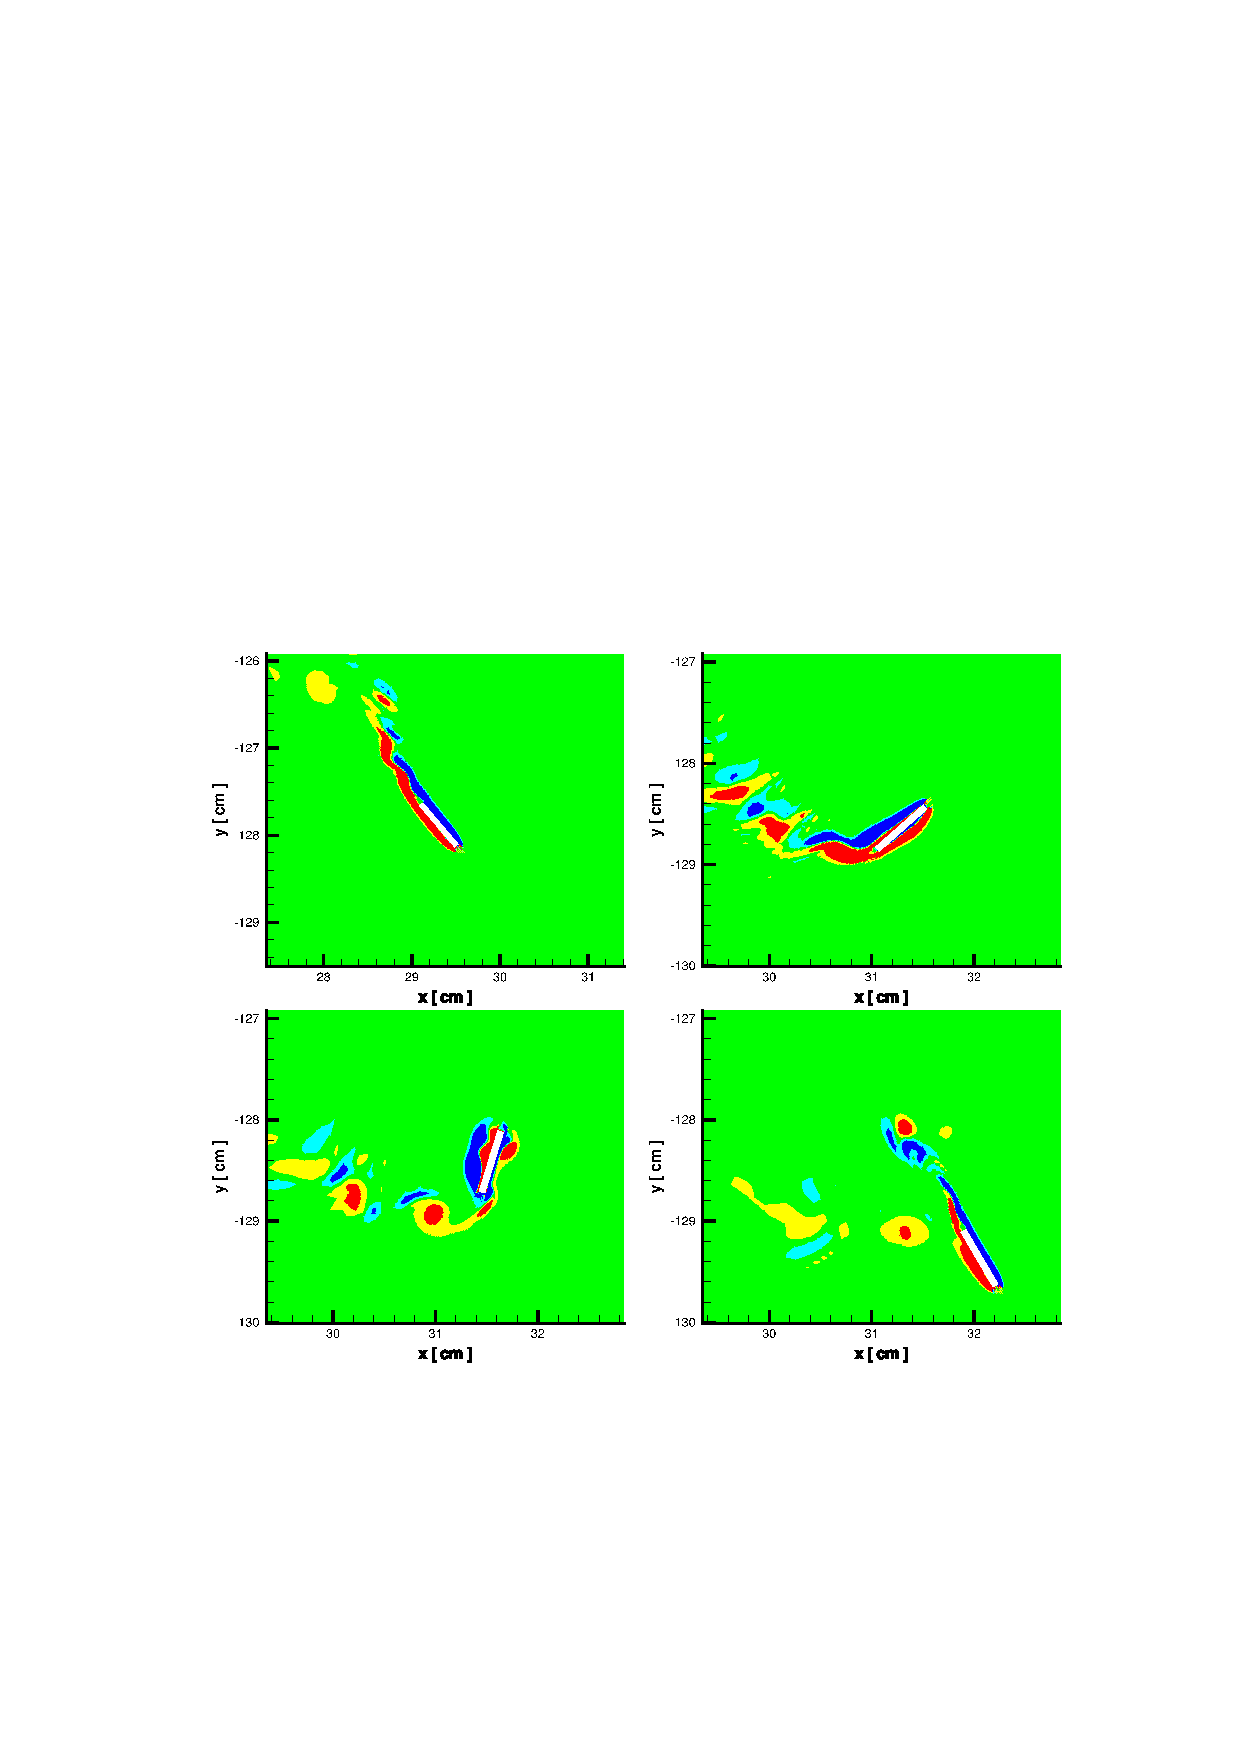
\includegraphics[height=.7\textheight]{FallingPlateVorticity.pdf}
    \caption{Vorticity of a freely falling plate at four instants
      during a full rotation\cite{jin08}}
  \end{figure}
\end{frame}

\section{The Unified Coordinates Method}

\subsection{Theoretical Background}

\begin{frame}{The Unified Coordinate Transformation}

\begin{align}
\label{eq:coordinate_transformation}
\left(
\begin{array}{c}
dt\\dx\\dy\\dz
\end{array}
\right) &= \left(
\begin{array}{cccc}
1 & 0 & 0 & 0 \\
U & A & L & P \\
V & B & M & Q \\
W & C & N & R \end{array} \right)
\left( \begin{array}{c}
d\lambda\\d\xi\\d\eta\\d\zeta \end{array} \right)
\end{align}

The method of implementation is what separates the unified coordinate
system (UCS) from the arbitrary-Lagrangian-Eulerian system (ALE).

\end{frame}

\begin{frame}{Conservation Equations in Two Dimensions}
\begin{equation}
\label{eq:conservation}
\frac{\partial \bf{E}}{\partial \lambda} + \frac{\partial \bf{F}}{\partial \xi} + \frac{\partial \bf{G}}{\partial \eta} = 0
\end{equation}
{\small
\begin{equation}
\label{eq:vectors}
\resizebox{.9\hsize}{!}{$\bf{E} = \left(
\begin{array}{c}
\rho J \\
\rho J u \\
\rho J v \\
\rho J e \\
A \\
B \\
L \\
M 
\end{array}
\right)
,
\bf{F} = \left(
\begin{array}{c}
\rho J \left( u_\xi - U_\xi \right) \\
\rho J \left( u_\xi - U_\xi \right) u + p M \\
\rho J \left( u_\xi - U_\xi \right) v - p L \\
\rho J \left( u_\xi - U_\xi \right) e + p J u_\xi \\
- U \\
- V \\
0 \\
0
\end{array}
\right)
,
\bf{G} = \left(
\begin{array}{c}
\rho J \left( u_\eta - U_\eta \right) \\
\rho J \left( u_\eta - U_\eta \right) u - p B \\
\rho J \left( u_\eta - U_\eta \right) v + p A \\
\rho J \left( u_\eta - U_\eta \right) e + p J u_\eta\\
0 \\
0 \\
- U \\
- V
\end{array}
\right)$}
\end{equation}
}
\begin{equation}
\label{eq:intermediates}
J = A M - B L , \,u_\xi = \frac{u M - v L}{J} , \,u_\eta = \frac{A v - B u}{J}
\end{equation}
\end{frame}

\begin{frame}{Controlling Grid Distortion}
  It is possible to preserve grid angles by requiring that $U$ satisfy
  an ODE: 
  \begin{equation}
    \resizebox{.9\hsize}{!}{$0=
    \frac{\partial}{\partial \tau}\left[\cos^{-1}\left(
        \frac{\nabla \xi \cdot \nabla \eta}{\left|\nabla
            \xi\right|\left|\nabla \eta\right|}
      \right)\right]
    =
    \frac{\partial}{\partial \tau}\left[\cos^{-1}\left(
        \frac{AL+BM}{\sqrt{A^2+B^2}\sqrt{L^2+M^2}}
      \right)\right]
    $}
  \end{equation}
  \begin{align}
    \Rightarrow 0=&~U_\eta 
    +\frac{S^2A}{T^2J}\left(Av_\xi-Bu_\xi\right)
    -\frac{L}{J}\left(Av_\eta-Bu_\eta\right)\\
    +&\left(\frac{S^2}{T^2J}\left(B_\xi \notag
        A+BA_\xi\right)-\frac{L}{JA}\left(B_\eta
        A+BA_\eta\right)\right)\left(U-u\right)
  \end{align}
\end{frame}

%\subsection{Algorithm}
%
%\begin{frame}[allowframebreaks]{The UCS Algorithm}
%The algorithm is given as follows. For each time step:
%
%\begin{enumerate}
%  \item Compute optimal time step\cite{huiviscous07}. Predict the maximum coordinate advancement of the first column of nodes. If necessary, limit the time step such that the first column ends the time step no more than $\Delta\xi$ from the upstream boundary, to prevent nonuniformity in the node spacing.
%  \item Apply Strang splitting, as above:
%  \begin{enumerate} 
%    \item Identify the appropriate time-advancement and the active interfaces for the given Strang step. Active interfaces are left/right for the $\xi$ steps of Strang splitting, and top/bottom for the $\eta$ step.
%    \item Step through nodes. For each node $n_{i,j}$:
%    \begin{enumerate}
%    \item Identify adjoining states using neighboring nodes, boundary conditions, and MUSCL interpolation, as appropriate.
%    \item Solve the local, one-dimensional Riemann problem to obtain the values of flow variables at the interface between adjoining states.
%    \item Use interfacial flow values and the value of $h$ that corresponds to the cell being updated to compute updated cell metric coefficients $A$, $B$, $L$, and $M$. Store all updated node values separately until after all nodes have been computed.
%    \item Compute physical flux into the cell using the values of flow variables at the interfaces and the updated geometric variables corresponding to the cell being updated.
%    \item Use flux to compute updated flow values. 
%    \end{enumerate}
%    \item Update all nodes.
%  \end{enumerate}
%  \item Solve for $h$ and update coordinate positions using trapezoidal integration.
%  \item Add/remove columns of nodes as needed.
%\end{enumerate}
%
%\end{frame}
%
\section{Results and Applications}

\subsection{Verification Problems}

\begin{frame}{The Riemann Problem}
  \begin{figure}
    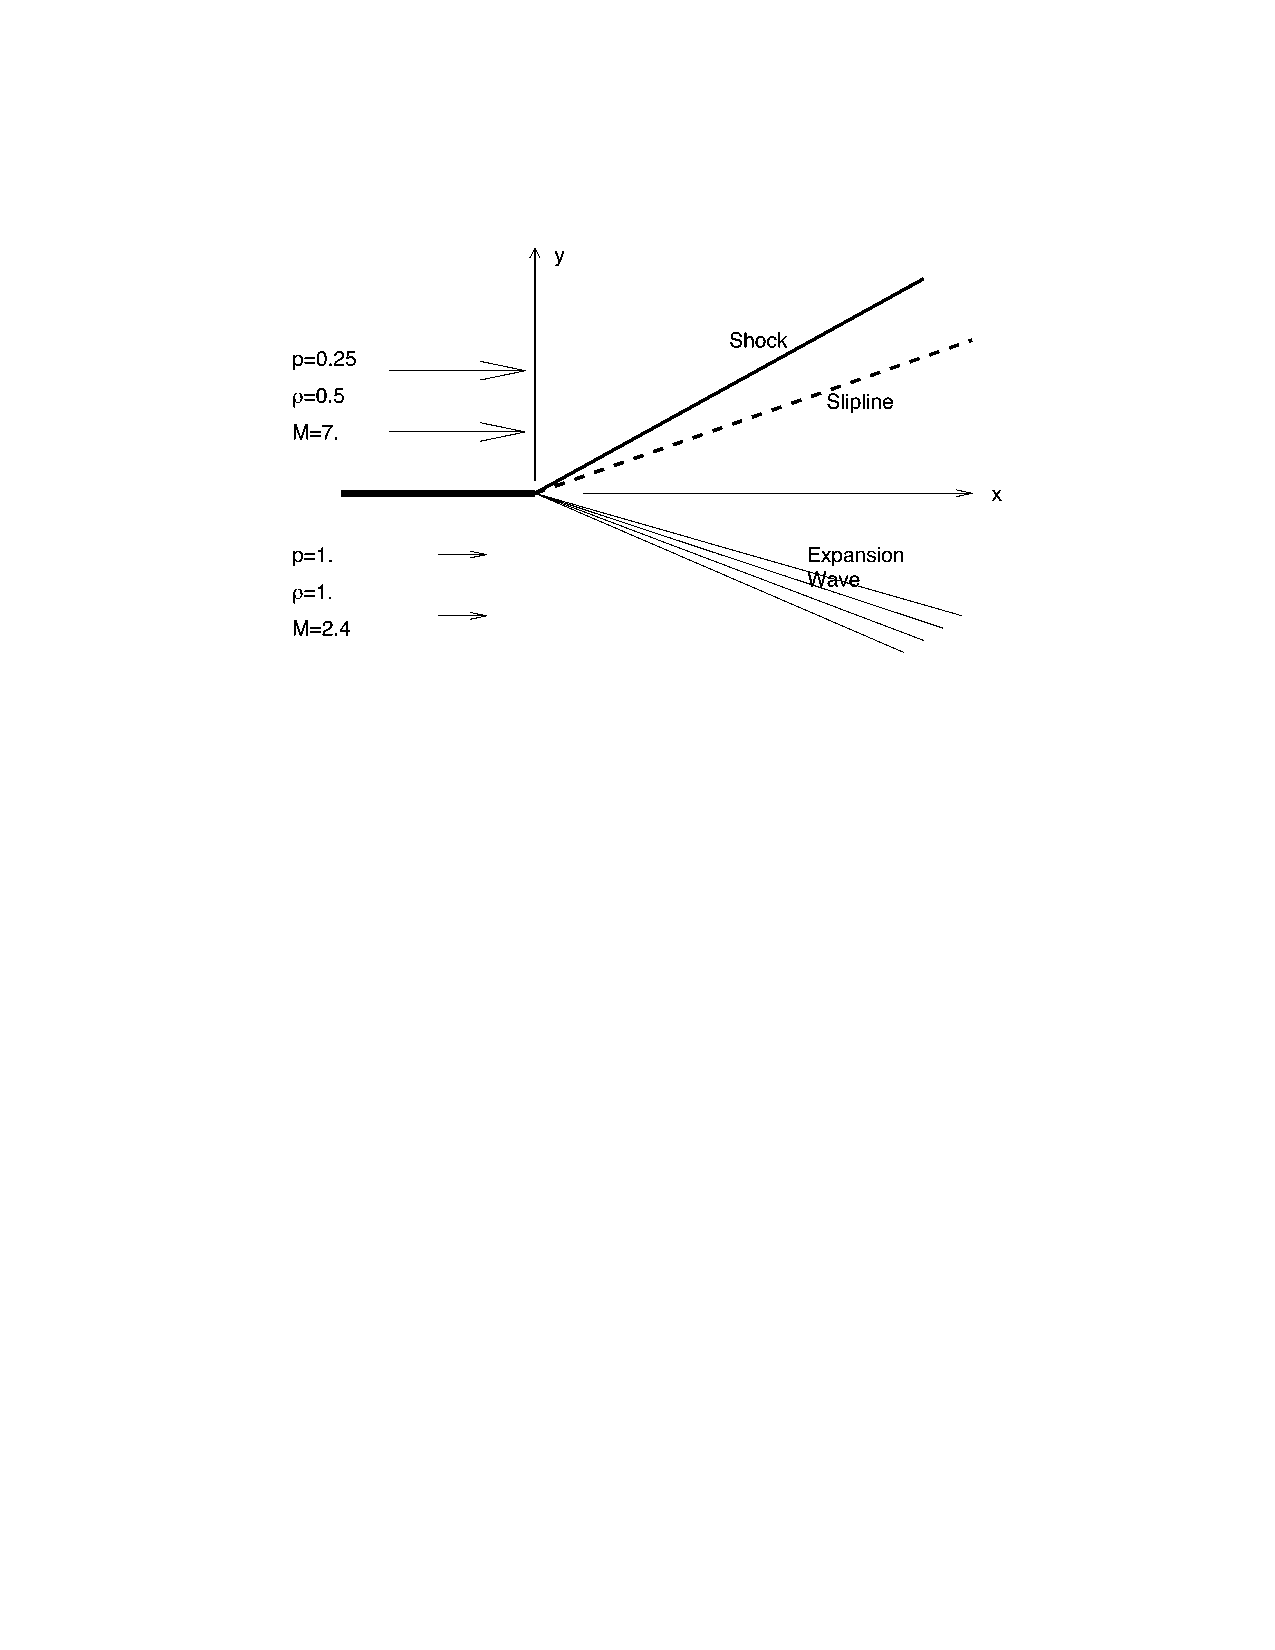
\includegraphics[height=.7\textheight]{steadyriemann.pdf}
    \caption{A diagram of the steady Riemann problem, as given by
      Hui\cite{hui99}}
  \end{figure}
\end{frame}

\begin{frame}{The Riemann Problem}
\begin{figure}[htbp]
   \centering
      \begin{subfigmatrix}{2}
        \subfigure[Eulerian coordinate system]{\label{fig:riemann_similarity_0}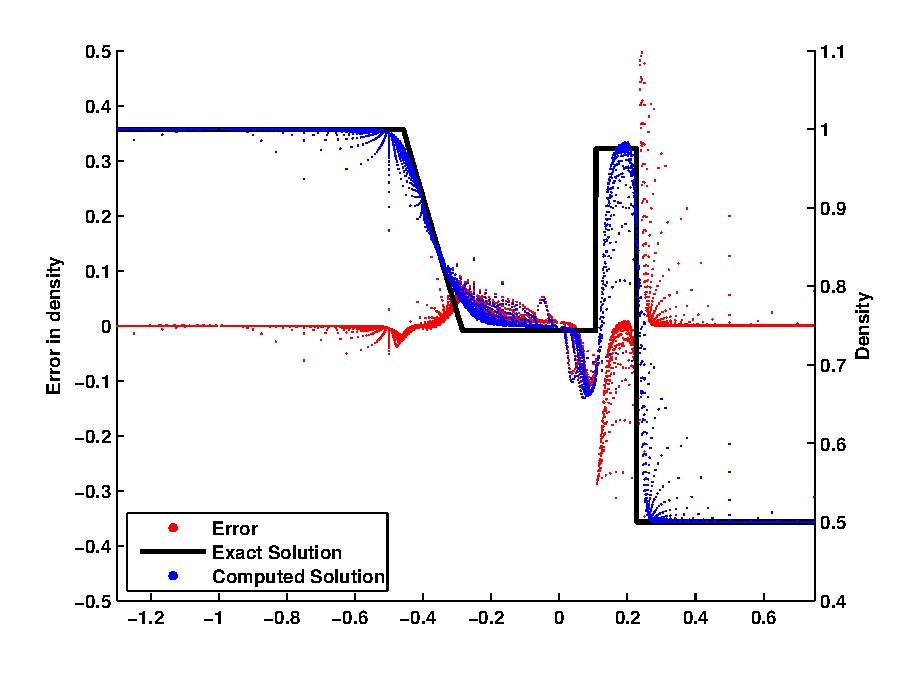
\includegraphics[width=.45\textwidth]{density_error_0.pdf}}
        \subfigure[Lagrangian coordinate system]{\label{fig:riemann_similarity_9}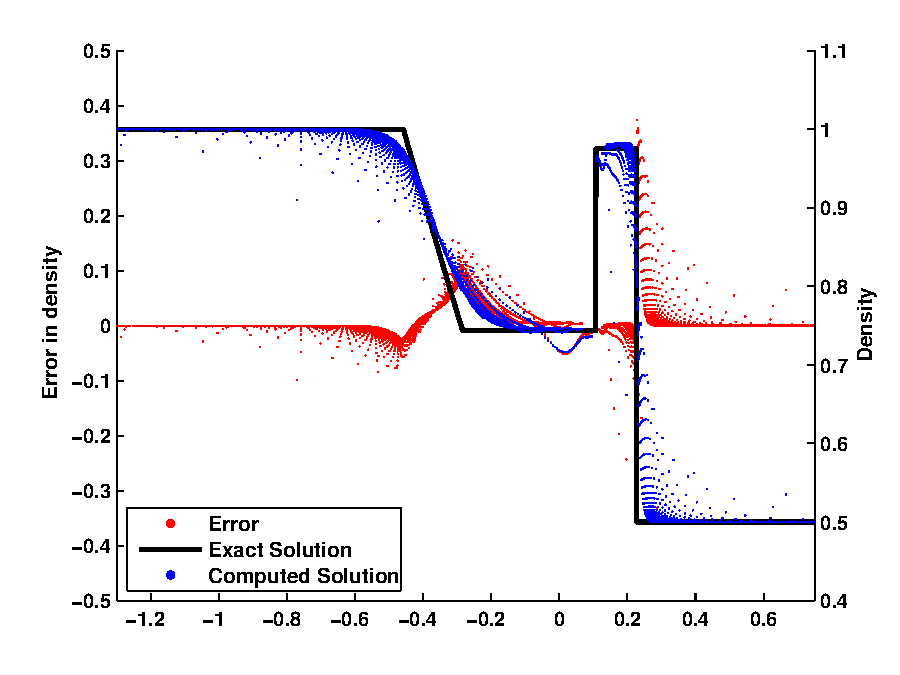
\includegraphics[width=.45\textwidth]{density_error_9.pdf}}
      \end{subfigmatrix}
   \caption{The similarity solution of the Riemann problem and the corresponding error in the numerical solution, computed throughout the simulation region.}
   \label{fig:riemann_similarity}
\end{figure}

\end{frame}

\begin{frame}{The Riemann Problem - Convergence}
\begin{figure}[htbp]%{r}{.6\textwidth}
   \centering
%   \vspace{-.25in}
   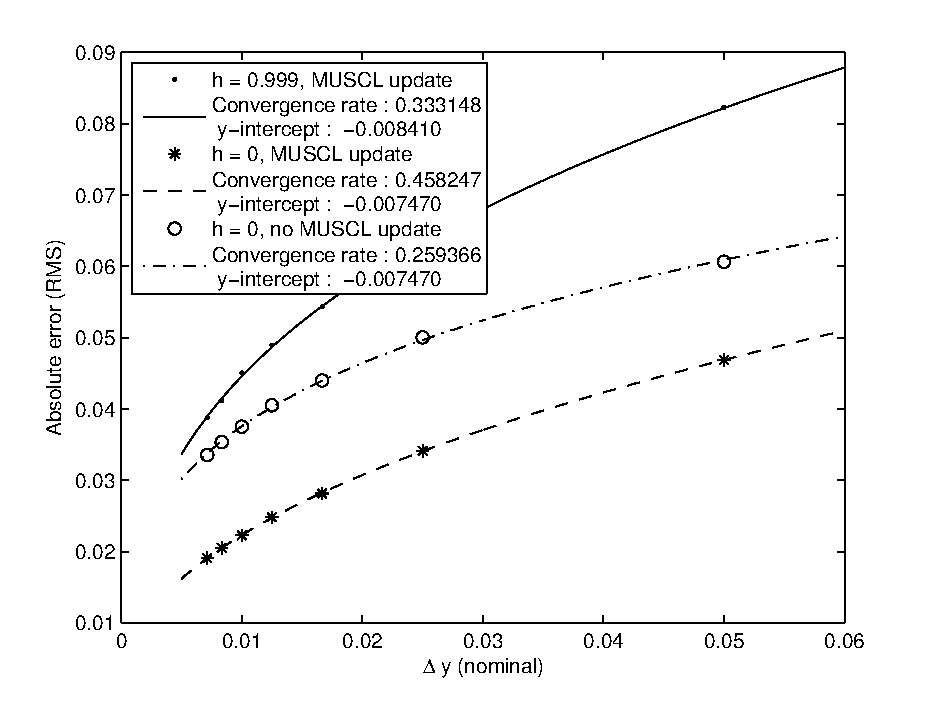
\includegraphics[width=.6\textwidth]{Riemann_convergence.pdf} 
   \caption{Root-mean-squared error for the riemann problem, with order of convergence $n$.}
   \label{fig:riemann_convergence}
%   \vspace{in}
\end{figure}
\end{frame}

% \begin{frame}{The Oblique Shock}
% \begin{figure}[htbp]
%    \centering
%    \begin{subfigmatrix}{2}
%     \subfigure[Root-mean-squared error for the oblique shock problem. The appearance of grid instabilities leads to two distinct error curves with different rates of convergence $n$.]{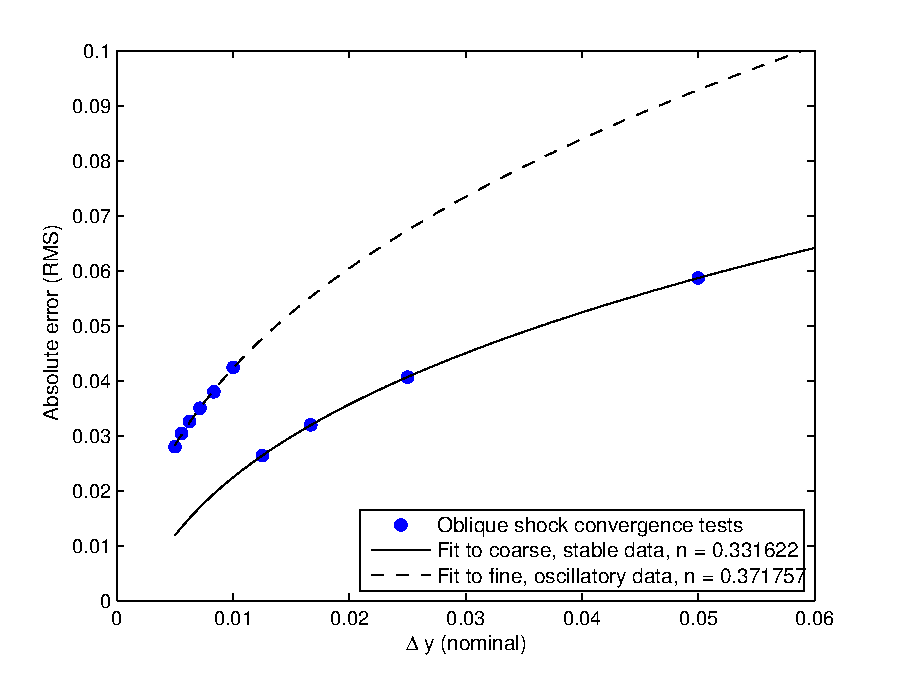
\includegraphics[width=.45\textwidth]{shock_convergence.pdf} }
%     \subfigure[A plot of normalized error in pressure, highlighting the oscillations which propogate downstream from the oblique shock.]{
%    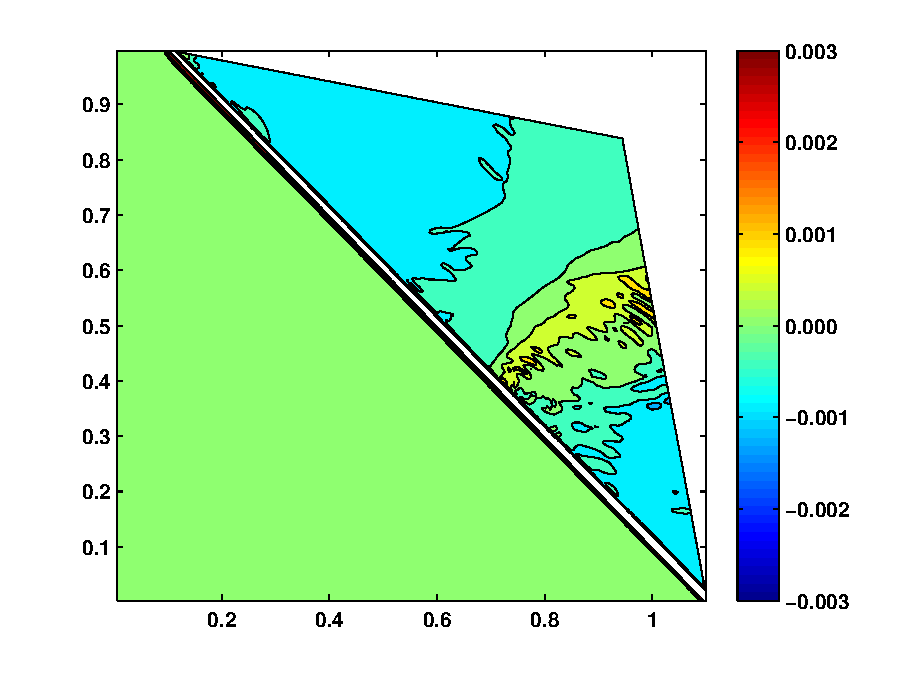
\includegraphics[width=.45\textwidth]{shock_instabilities.pdf}
%    \label{fig:shock_instabilities}}
%    \end{subfigmatrix}
%    \caption{The oblique shock wave}
% \end{figure}
% \end{frame}

\begin{frame}{The Expansion Corner}
\begin{figure}[htbp] %  figure placement: here, top, bottom, or page
   \centering
   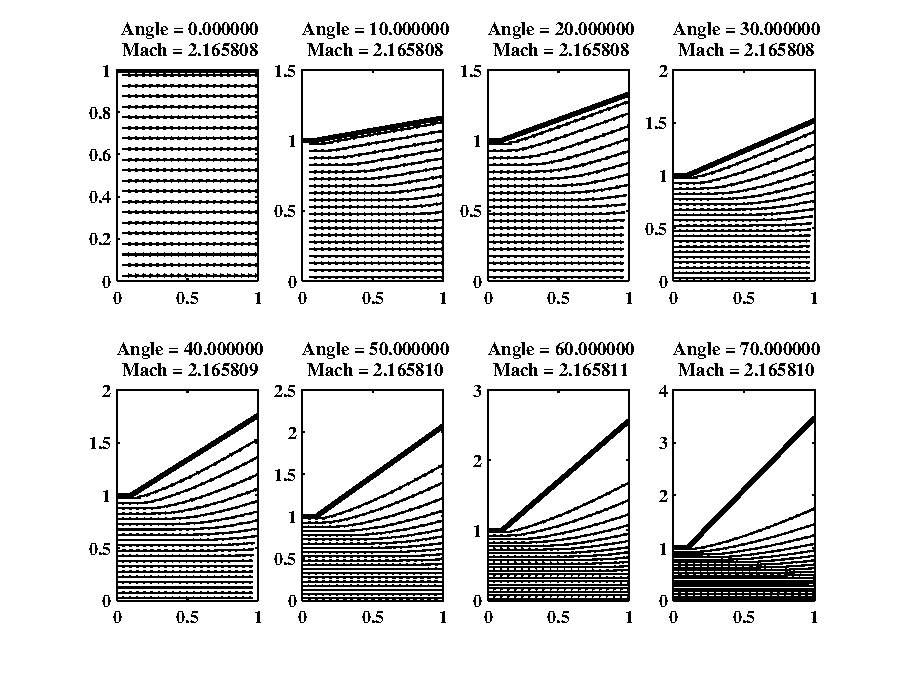
\includegraphics[height=.7\textheight]{Expansion.pdf} 
   \caption{Computed streamlines for Prandtl-Meyer expansion at increasing expansion angles. Angles are given in degrees. }
   \label{fig:expansion_separation}

\end{figure}

\end{frame}

\subsection{Demonstration Problems}

\begin{frame}{The Diamond Shock Train}
\begin{figure}[htbp]
   \centering
%   \vspace{-.5in}
   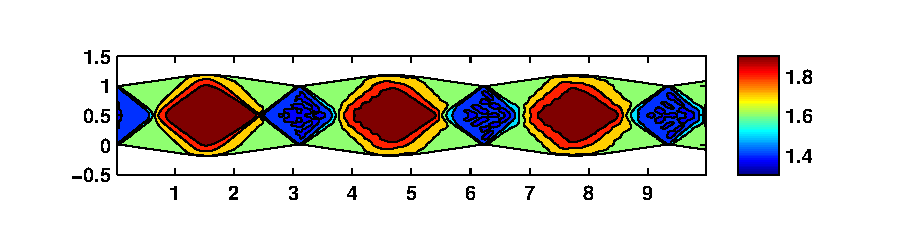
\includegraphics[width=\textwidth]{diamond_shock_train.pdf}
   \caption{Computed Mach number for an under-expanded nozzle flow,
     showing the diamond-shock train}
   \label{fig:nozzle_flow}
\end{figure}
\end{frame}

%\begin{frame}{The Isentropic Nozzle}
%\begin{figure}[htbp]
%   \centering
%   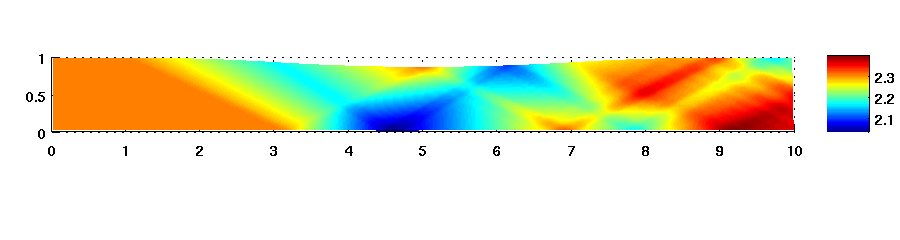
\includegraphics[width=\textwidth]{isentropic_nozzle1p0.pdf}
%   \caption{Computed Mach number for isentropic flow through a constricting, parabolic, supersonic channel}
%\end{figure}
%\end{frame}

\begin{frame}{The Transonic Duct}
\begin{figure}[htbp]
   \centering
   \begin{subfigmatrix}{2}
      \subfigure[$h=0$, nominal grid size: $72 \times 20$]{
   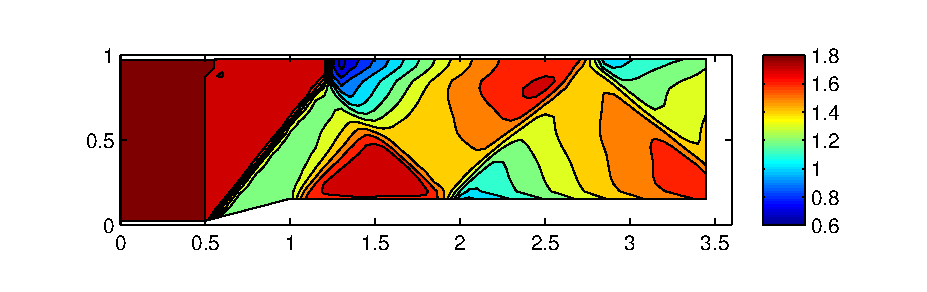
\includegraphics[height=.15\textheight]{shock_train_contourh00p4.pdf}
   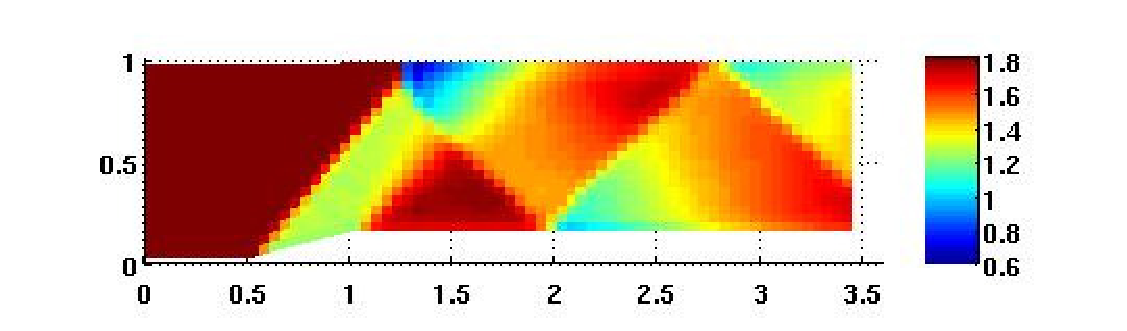
\includegraphics[height=.15\textheight]{shock_train_surfh00p4.pdf}}
      \subfigure[$h=0.25$, nominal grid size: $72 \times 20$]{
   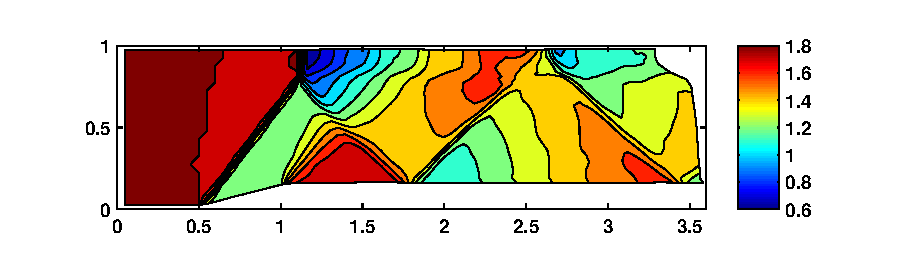
\includegraphics[height=.15\textheight]{shock_train_contourh250p4.pdf}
   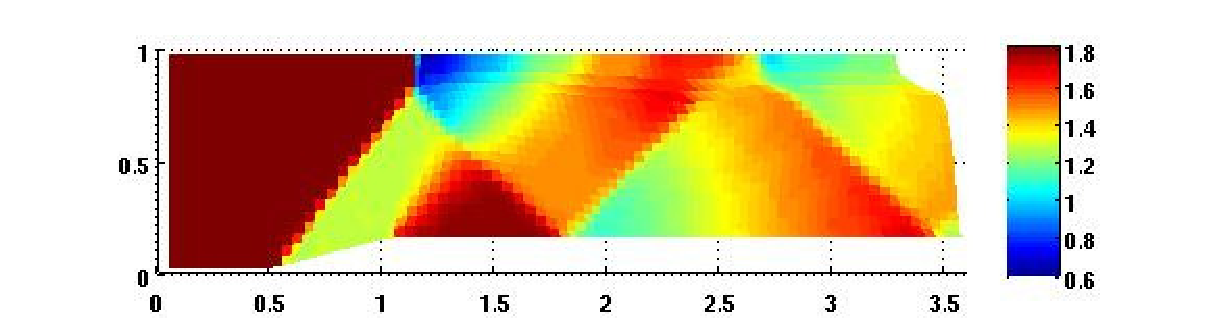
\includegraphics[height=.15\textheight]{shock_train_surfh250p4.pdf}}
      \subfigure[$h=0$, nominal grid size: $360 \times 100$]{
   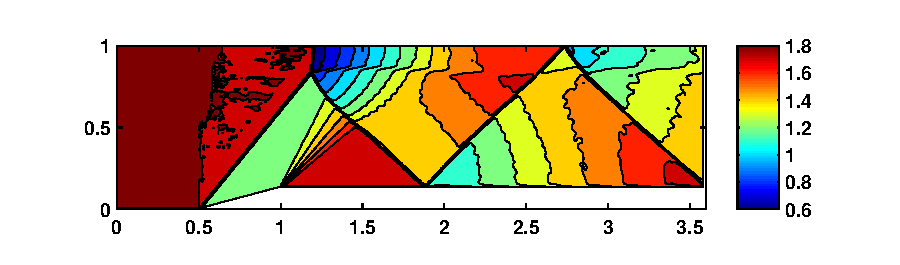
\includegraphics[height=.15\textheight]{shock_train_contourh02p0.pdf}
   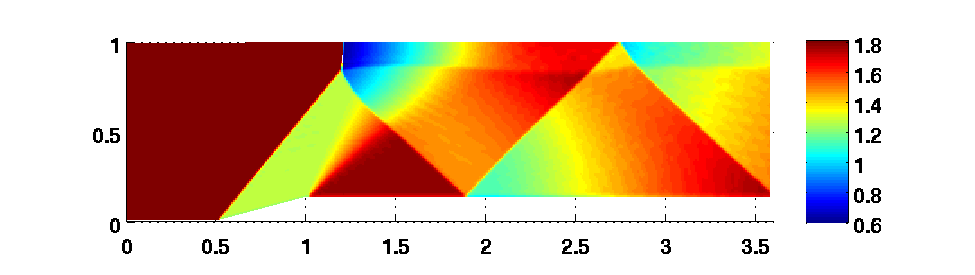
\includegraphics[height=.15\textheight]{shock_train_surfh02p0.pdf}}
   \end{subfigmatrix}
   \caption{Qualitative accuracy comparison between UCS and Eulerian simulations for a transonic duct flow. Notice the improved resolution of the slip line and the walls for the UCS solution.}
   \label{fig:duct_verification}
\end{figure}
\end{frame}

\begin{frame}{Boundary-layer flow}
\begin{figure}[htbp]
   \centering
   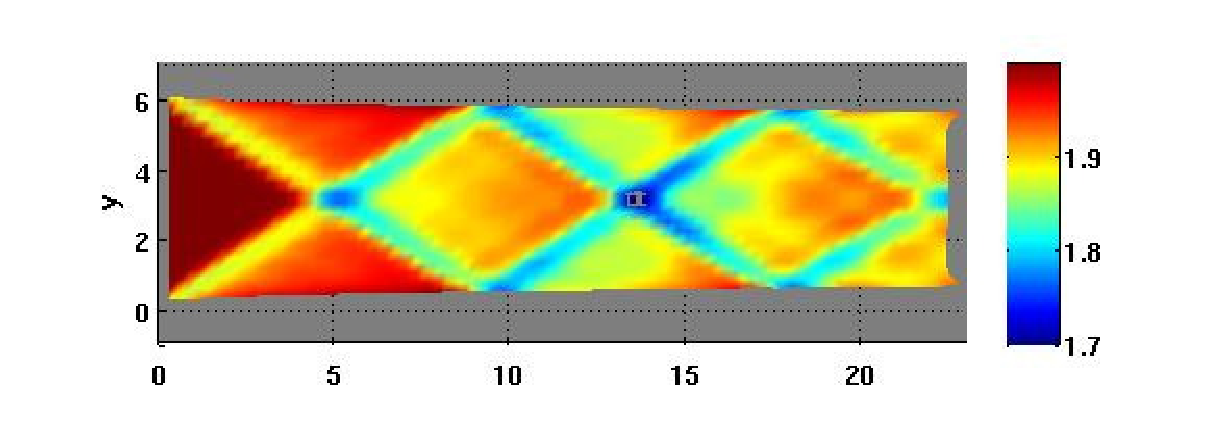
\includegraphics[width=\textwidth]{BL_shock_train.pdf}
   \caption{Oblique shock train produced by a turbulent boundary layer in an otherwise uniform channel}
   \label{fig:bl_shock_train}
\end{figure}
\end{frame}

\begin{frame}{A more interesting application}
\begin{figure}
%   \centering
   \vspace{-.65in}
   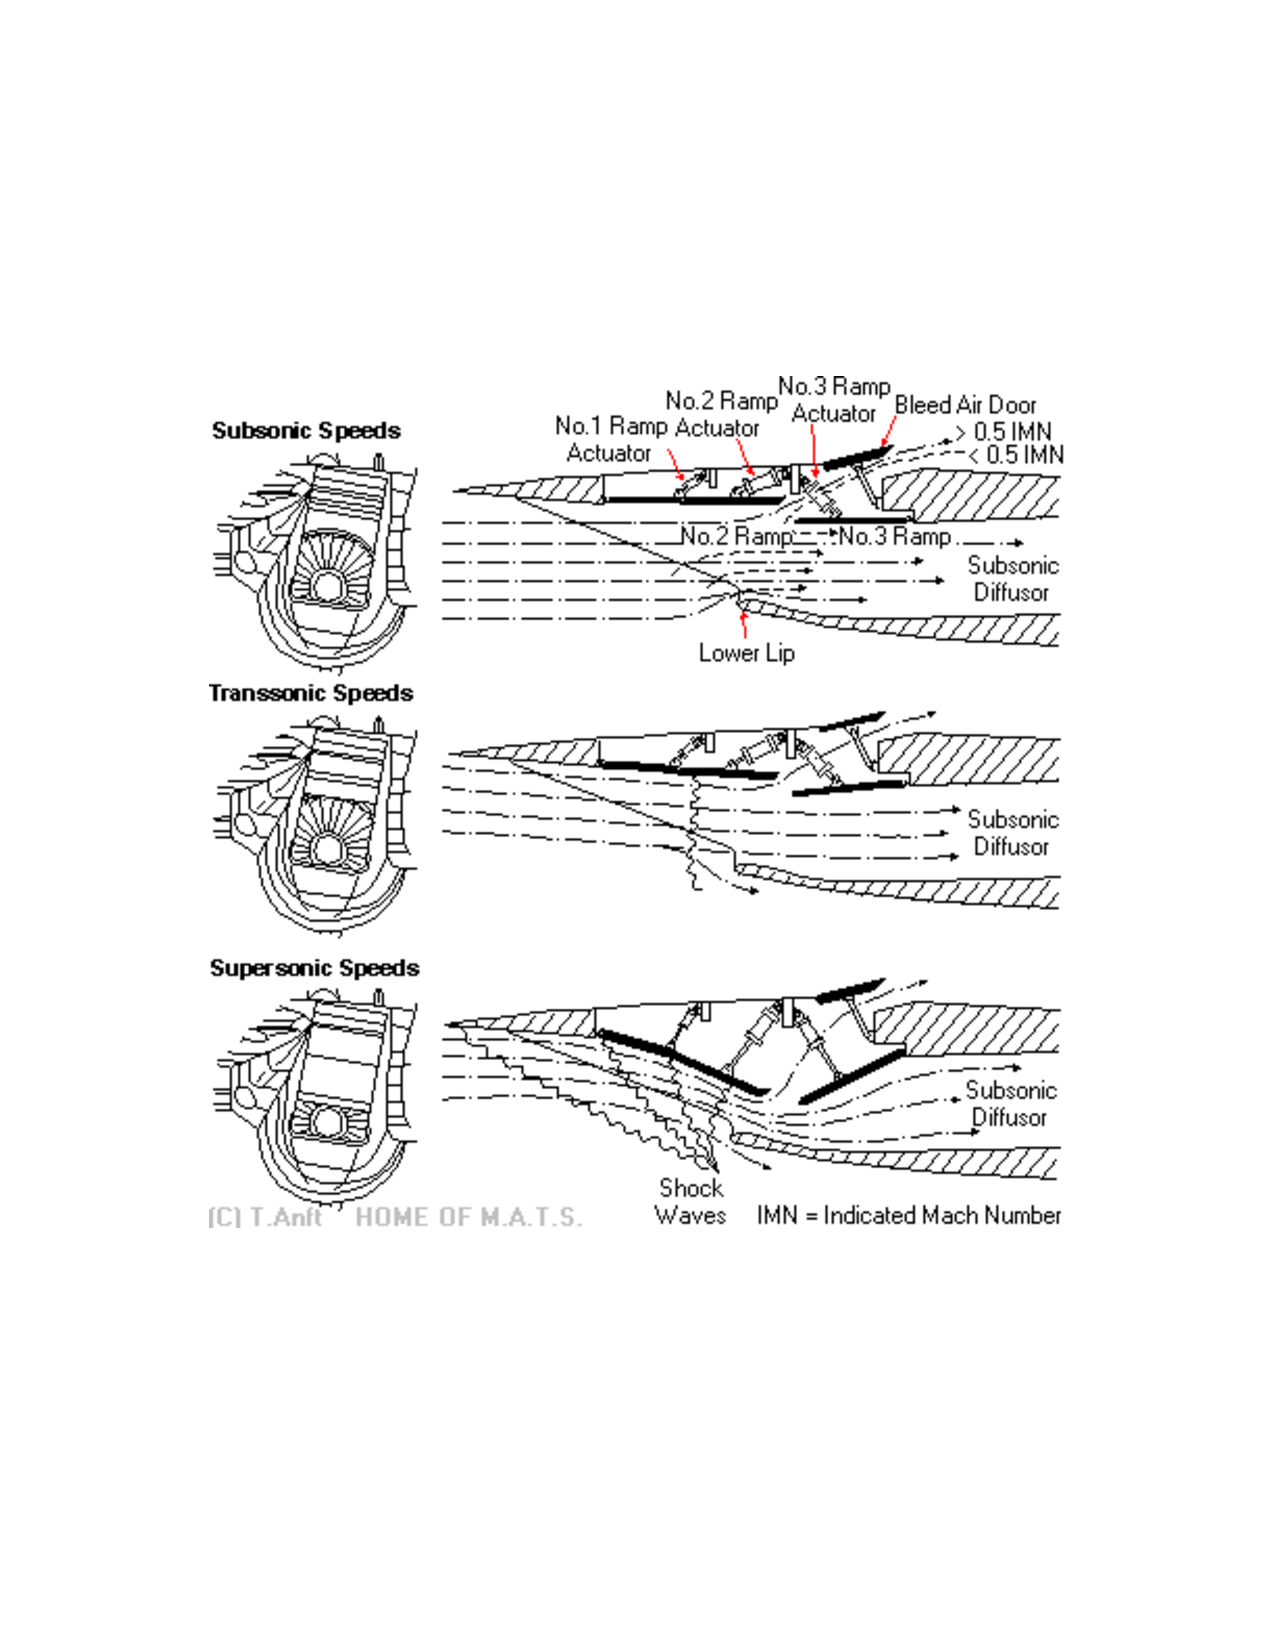
\includegraphics[height=\textheight]{F_14_inlet_diagram.pdf}
   \vspace{-.65in}
   \caption{Diagram of the variable inlet geometry of the USAF F-14 Tomcat. Courtesy Home of M.A.T.S., http://www.anft.net/f-14/f14-detail-airintake.htm}
   \label{fig:f-14_diagram}
\end{figure}
\end{frame}

\begin{frame}{A more interesting application}
\begin{figure}[htbp]
   \centering
   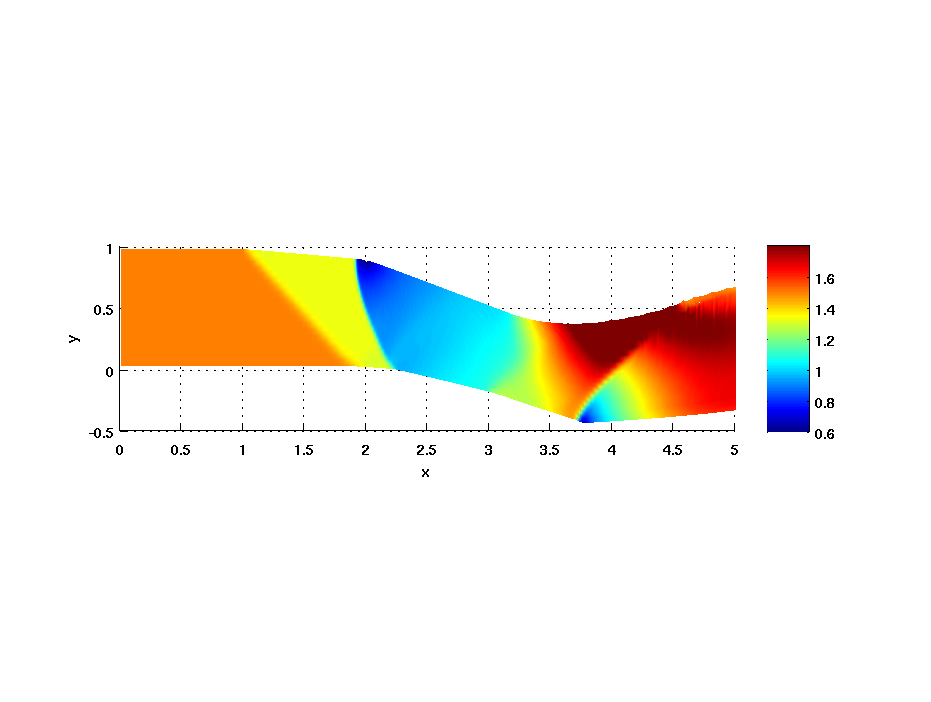
\includegraphics[width=\textwidth]{F_14_filmstrip_5clean.pdf}
   \caption[Mach Number in F-14 Inlet]{Mach number in a geometry modeled after Fig.~\ref{fig:f-14_diagram}.}
   \label{fig:f-14_flow}
\end{figure}
\end{frame}

\section{Proposal}

\begin{frame}{Timeline}
  \begin{figure}
    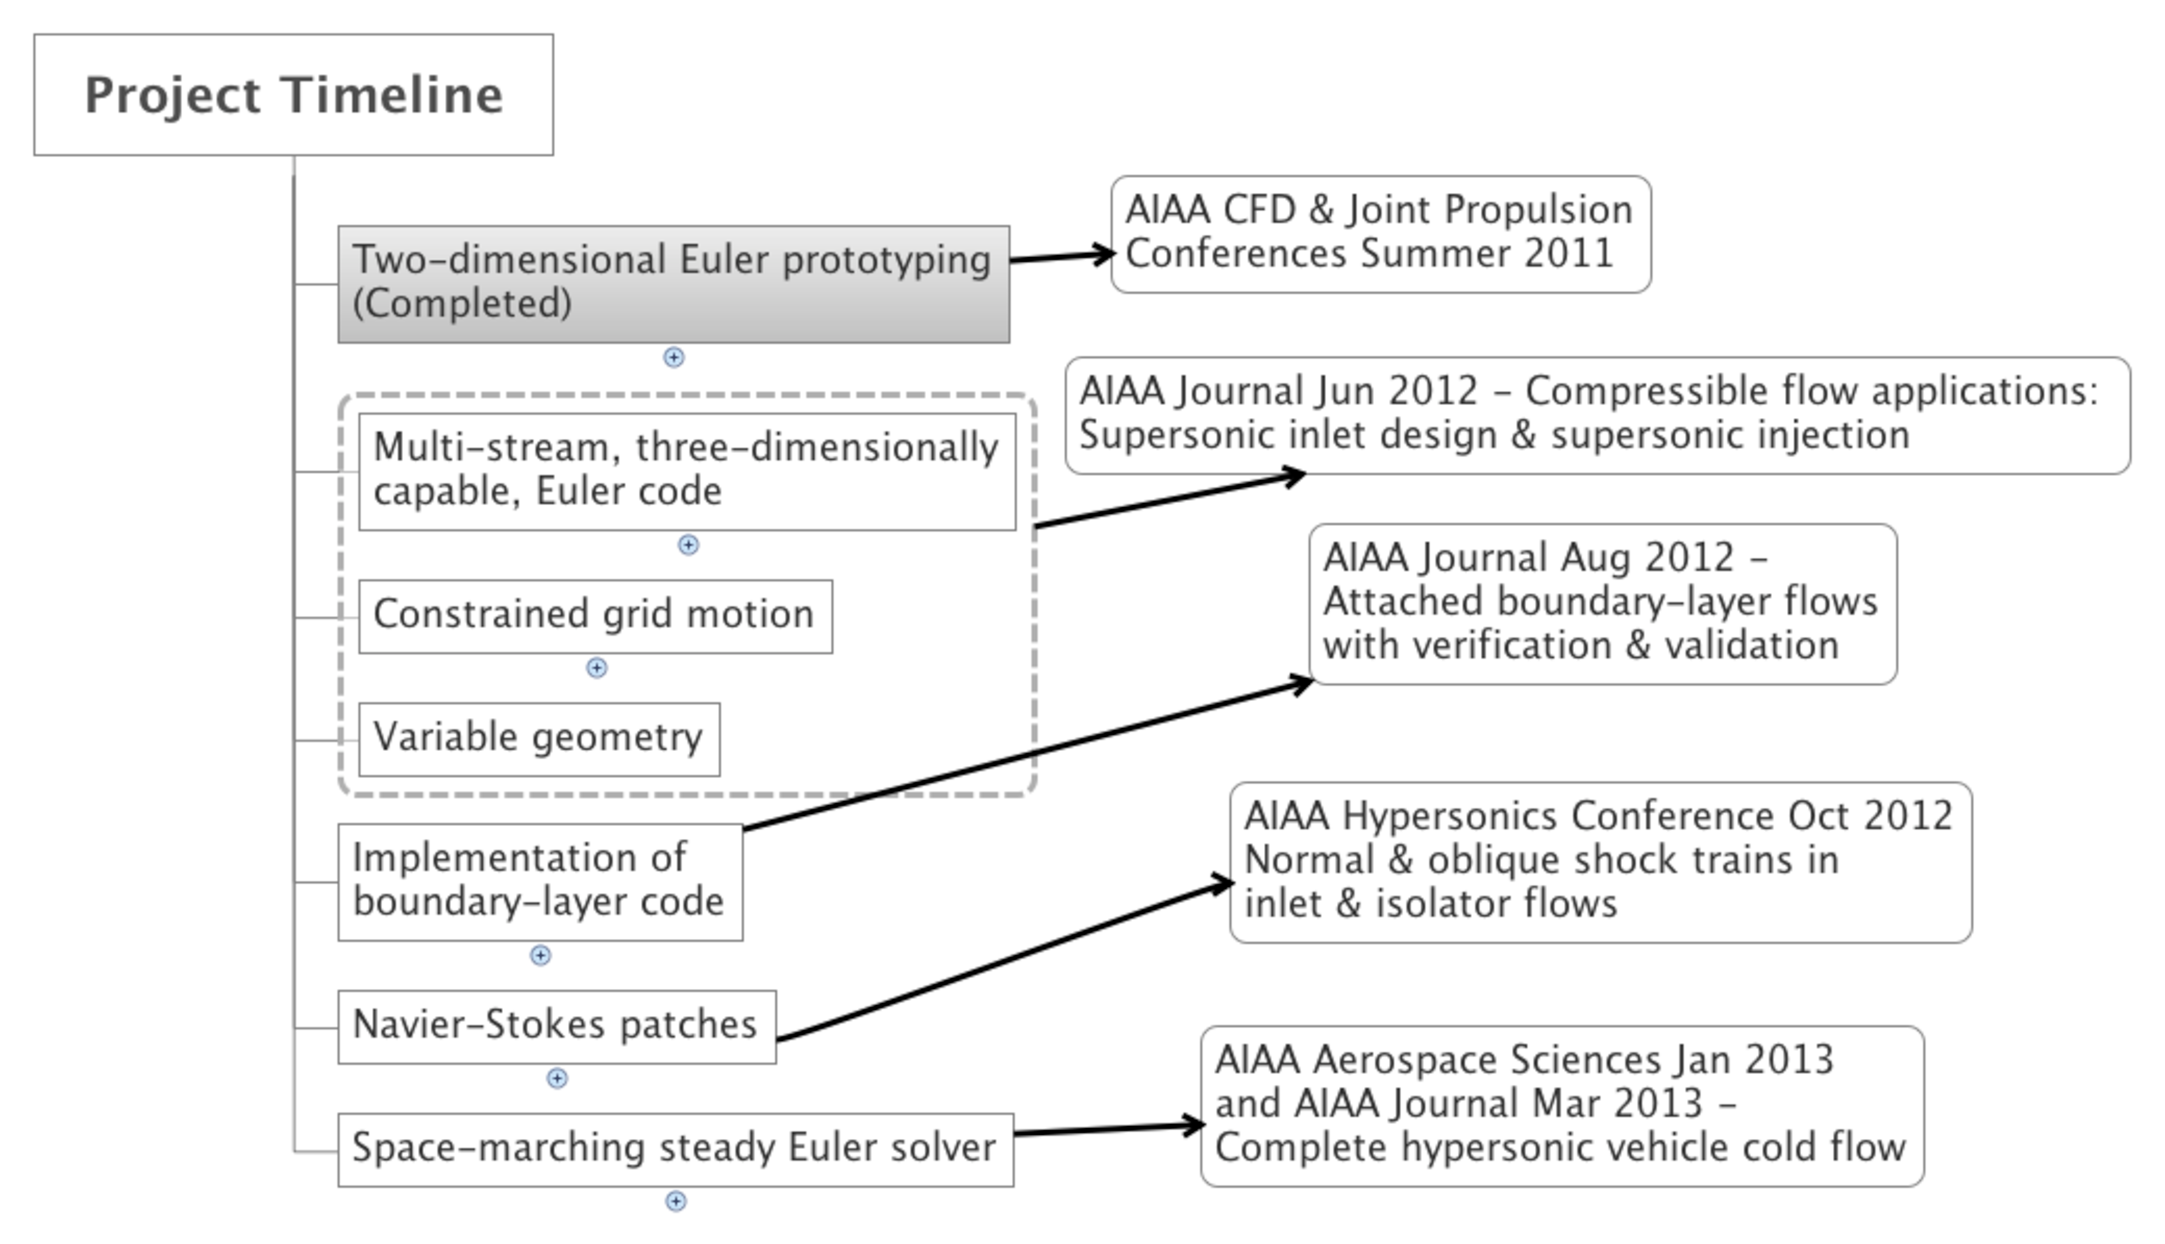
\includegraphics[width=\textwidth]{Timeline.pdf}
  \end{figure}
\end{frame}

% \begin{frame}{Euler Solver \& Multi-Stream Framework}

% \section{Summary}

% \begin{frame}{Summary}

%   % Keep the summary *very short*.
%   \begin{itemize}
%   \item
%     The major advantage of UCS is the automatic mesh
%   \item
%     UCS must be implemented in a way that improves stability and accuracy
%   \end{itemize}
  
%   % The following outlook is optional.
%   \vskip0pt plus.5fill
%   \begin{itemize}
%   \item
%     Future Work
%     \begin{itemize}
%     \item
%       Optimize for speed
%     \item
%       Boundary layer solver
%     \item
%       Shock-aligned grid
%     \end{itemize}
%   \end{itemize}
% \end{frame}



% All of the following is optional and typically not needed. 
%\appendix
%\section<presentation>*{\appendixname}
%\subsection<presentation>*{For Further Reading}

\begin{frame}[allowframebreaks]
  \frametitle<presentation>{References and Further Reading}
    
%  \begin{thebibliography}{10}
%    
%  \beamertemplatebookbibitems
%  % Start with overview books.
%
%  \bibitem{V_diagram}
%    Washington State Department of Transportation
%    \newblock {\em Systems Engineering for Intelligent Transportation Systems}
%    \newblock Dec. 30, 2005. (Retrieved from Wikimedia Commons)
%
%  \bibitem{Author1990}
%    A.~Author.
%    \newblock {\em Handbook of Everything}.
%    \newblock Some Press, 1990.
% 
%    
%  \beamertemplatearticlebibitems
  % Followed by interesting articles. Keep the list short. 
%
%  \bibitem{Someone2000}
%    S.~Someone.
%    \newblock On this and that.
%    \newblock {\em Journal of This and That}, 2(1):50--100,
%    2000.
%  
%  \end{thebibliography}

  \bibliographystyle{aiaa}
  \bibliography{Project}

\end{frame}

\end{document}

